% include the page wise photos of plagarism summary document:
% \chapter{MATHEMATICAL DERIVATIONS}
% You can include the Derivation and mathematical part of your project that is not necessary to be included in the main report here. To provide reader with the complete mathematical background of your project, you can include the derivations, proofs, and detailed explanations of theorems or formulas used in your project. and then you can cross reference them in the main report.
% \section{Proof of Theorem 1:} Convex Optimization Problem can be solved using Gradient Descent Method.
% \section{Proof of Theorem 2:} Convergence of Gradient Descent Method for Convex Functions.
% \section{Gaussian Distribution} 
% The Gaussian distribution, also known as the normal distribution, is a continuous probability distribution characterized by its bell-shaped curve. It is defined by its mean ($\mu$) and standard deviation ($\sigma$). The probability density function (PDF) of a Gaussian distribution is given by:
% \[
% f(x) = \frac{1}{\sigma\sqrt{2\pi}} \exp\!\left(-\frac{(x-\mu)^2}{2\sigma^2}\right).
% \]
\chapter{APPENDICES}
\section{PROJECT BUDGET}
\begin{table}[h!]
\centering
\caption{Estimated Project Budget for MotionBridge}
\label{tab:budget}
\renewcommand{\arraystretch}{1.2}
\small
\begin{tabular}{c l c r r}
\toprule
\textbf{S.N.} & \textbf{Qty} & \textbf{Unit Price (NPR)} & \textbf{Total Price (NPR)} \\
\midrule
1 & USB Webcams & 3 & 4000 & 12000 \\
2 & Camera Tripods & 3 & 1,500 & 4,500 \\
3 & Powered USB Hub & 1 & 2,000 & 2,000 \\
4 & Calibration Target & 1 & 1,000 & 1,000 \\
5 & Software \& Tools & - & - & Free \\
6 & Project Documentation & - & 2,500 & 2,500 \\
7 & Contingency Fund & - & 2,000 & 2,000 \\
\midrule
\multicolumn{4}{r}{\textbf{Total Estimated Budget:}} & \textbf{NPR 24,000} \\
\bottomrule
\end{tabular}
\end{table}

\section{PROJECT TIMELINE}
\subsection{Gantt Chart}
% \textbf{Gantt Chart Placeholder here:}
\begin{table}[H]
    \centering
    \caption{Gantt Chart for Project Timeline}
    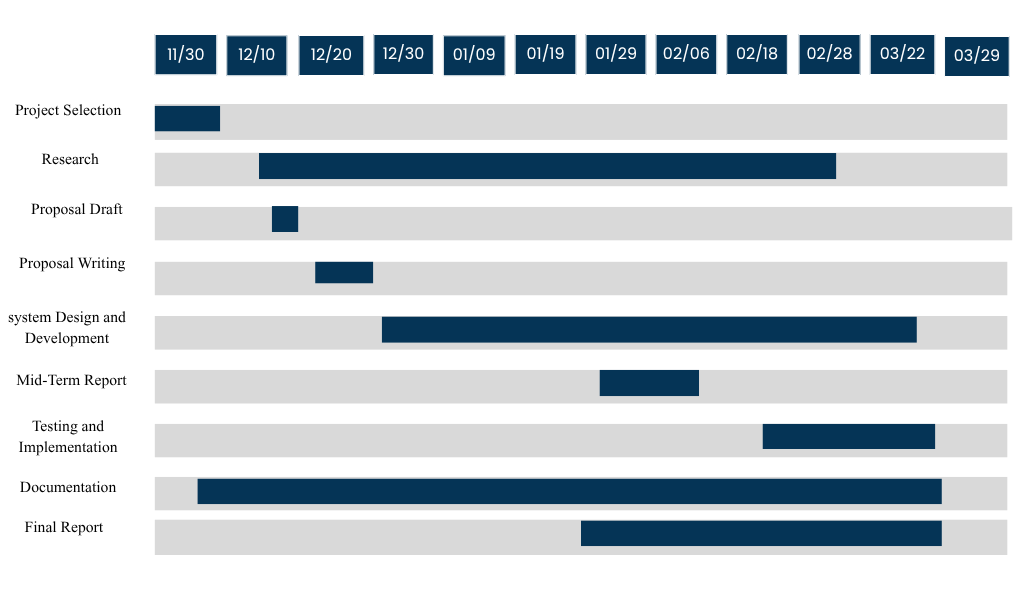
\includegraphics[width=\textwidth]{src/images/Ganntchart.png}
    \label{tab:gantt_chart}
\end{table}
% \chapter{IMPLEMEMNTED CODE}
